% Proposta D (12/11/2026, pedido do autor): mais simples e didática que a C.
% O caminho principal (setas cheias, no centro) é o da operação indicada pelo
% ARIMA. O GARCH fica ao lado e só informa o risco (setas tracejadas): ao filtro,
% que decide se a operação é feita, e ao tamanho da posição. Assim a direção não
% entra no losango, e o losango tem uma pergunta só. Sem a fórmula do ajuste:
% "menor quanto maior o risco" é o que o Cap. I diz (volatility targeting).
% Mesmo estilo das fig05/fig06. Fora do TG até o autor decidir.
\documentclass[11pt,border=2pt]{standalone}
\usepackage[T1]{fontenc}
\usepackage[utf8]{inputenc}
\usepackage{mathptmx}
\usepackage{tikz}
\usetikzlibrary{arrows.meta,positioning,calc,shapes.geometric}
\tikzset{
  seta/.style={-{Stealth[length=2.2mm]}, semithick},
  info/.style={-{Stealth[length=2.2mm]}, semithick, dashed},
  caixa/.style={rectangle, draw, semithick, fill=gray!10, rounded corners=2pt,
                align=center, minimum width=46mm, minimum height=10mm, font=\small},
  dado/.style={trapezium, trapezium left angle=75, trapezium right angle=105, draw,
               semithick, fill=white, align=center, minimum height=9mm, font=\small,
               trapezium stretches body},
  decisao/.style={diamond, draw, semithick, fill=white, aspect=2.4, align=center,
                  inner sep=1pt, font=\small},
  pergunta/.style={font=\small\itshape, align=center},
  pequeno/.style={font=\footnotesize, align=center},
}
\begin{document}
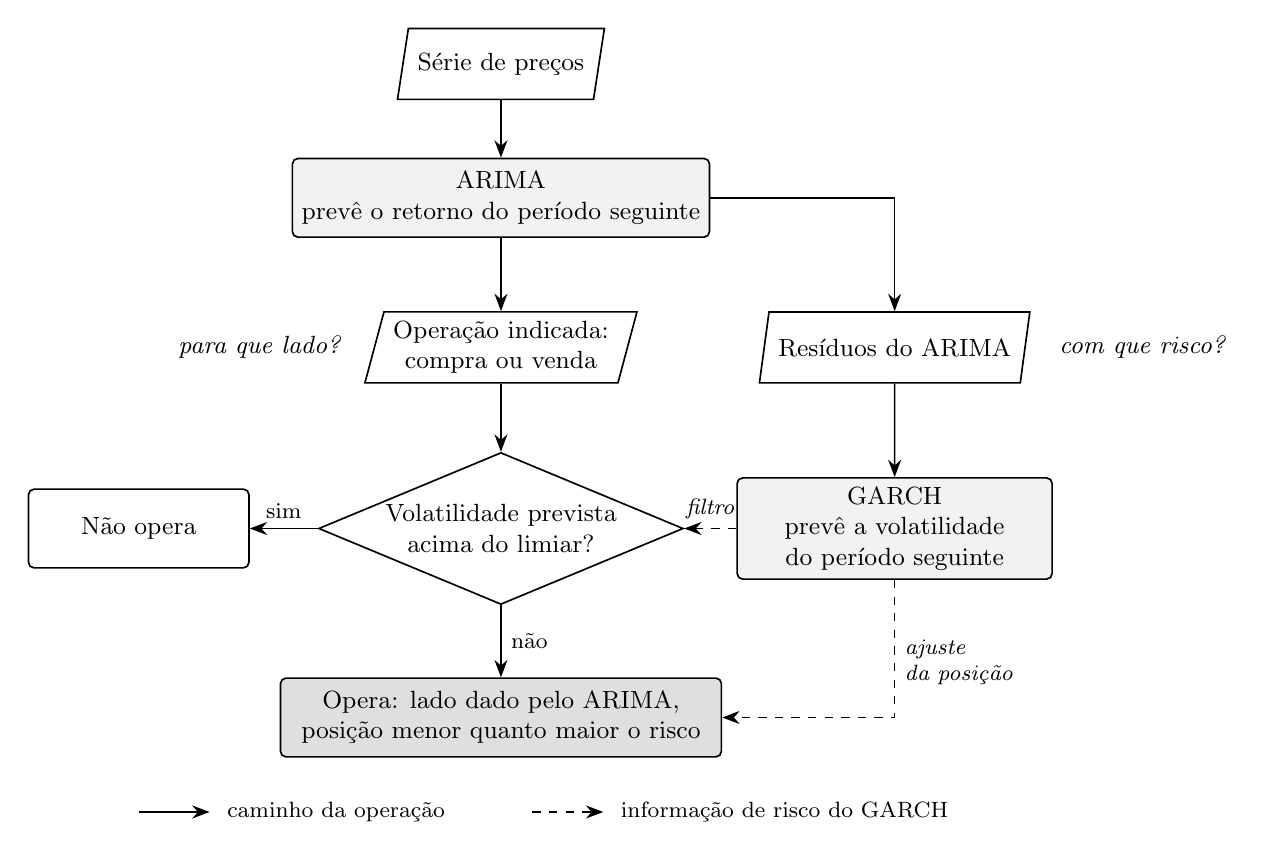
\begin{tikzpicture}
  % caminho da operação, no centro
  \node[dado] (ent) at (0,0) {Série de preços};
  \node[caixa] (arima) at (0,-1.7) {ARIMA\\prevê o retorno do período seguinte};
  \node[dado] (dir) at (0,-3.6) {Operação indicada:\\compra ou venda};
  \node[decisao] (lim) at (0,-5.9) {Volatilidade prevista\\acima do limiar?};
  \node[caixa, minimum width=28mm, fill=white] (veto) at (-4.6,-5.9) {Não opera};
  \node[caixa, fill=gray!25, minimum width=56mm] (op) at (0,-8.3)
    {Opera: lado dado pelo ARIMA,\\posição menor quanto maior o risco};

  % o GARCH, ao lado, informando o risco
  \node[dado] (res) at (5.0,-3.6) {Resíduos do ARIMA};
  \node[caixa, minimum width=40mm] (garch) at (5.0,-5.9) {GARCH\\prevê a volatilidade\\do período seguinte};

  \draw[seta] (ent) -- (arima);
  \draw[seta] (arima) -- (dir);
  \draw[seta] (dir) -- (lim);
  \draw[seta] (lim) -- node[above, pequeno]{sim} (veto);
  \draw[seta] (lim) -- node[right, pequeno]{não} (op);
  \draw[seta] (arima.east) -| (res.north);
  \draw[seta] (res) -- (garch);
  \draw[info] (garch) -- node[above, font=\footnotesize\itshape]{filtro} (lim);
  \draw[info] (garch.south) |- node[pos=0.3, right, font=\footnotesize\itshape, align=left]{ajuste\\da posição} (op.east);

  % as duas perguntas que a integração separa (Cap. I, 2º parágrafo da seção)
  \node[pergunta, anchor=east] at ([xshift=-3mm]dir.west) {para que lado?};
  \node[pergunta, anchor=west] at ([xshift=3mm]res.east) {com que risco?};

  % legenda
  \begin{scope}[shift={(-4.6,-9.5)}]
    \draw[seta] (0,0) -- (0.9,0); \node[pequeno, anchor=west] at (1.0,0) {caminho da operação};
    \draw[info] (5.0,0) -- (5.9,0); \node[pequeno, anchor=west] at (6.0,0) {informação de risco do GARCH};
  \end{scope}
\end{tikzpicture}
\end{document}
